% Arquivo editável que gera o pdf
% Copyright (C) 2018  Daniel Saad Nogueira Nunes (daniel.nunes@ifb.edu.br)

% This program is free software: you can redistribute it and/or modify
% it under the terms of the GNU General Public License as published by
% the Free Software Foundation, either version 3 of the License, or
% (at your option) any later version.

% This program is distributed in the hope that it will be useful,
% but WITHOUT ANY WARRANTY; without even the implied warranty of
% MERCHANTABILITY or FITNESS FOR A PARTICULAR PURPOSE.  See the
% GNU General Public License for more details.

% You should have received a copy of the GNU General Public License
% along with this program.  If not, see <http://www.gnu.org/licenses/>.


\documentclass{apresentacao-ifb}


% Insira os dados aqui
\author{Marcos Bezerra Campos}
\title{Extração de características em SNORNAs usando modelos matemáticos}
\subtitle{}
\institute{Instituto Federal de Brasília, Campus Taguatinga}
\date{2022}

\begin{document}
\maketitle



\section{Introdução}

\begin{frame}{Aprendizado de máquina em sequências genômicas}
    A expansão do Aprendizado de Máquina e de técnicas biológicas para a predição de
estruturas protéicas e genômicas trouxe um resultado significado no que tange a identificação de padrões e características em RNAs não-codificadores (ncRNAs). Pode ser dividido em duas vertentes:

    \begin{itemize}
        \item Aprendizado de máquina supervisionado
        \item Aprendizado de máquina não-supervisionado
    \end{itemize}
\end{frame}

\section{Introdução}

\begin{frame}{snoRNAs}
	Em uma sequência de \textit{ncRNA}, é possível identificar pequenas moléculas de RNAs nucleolares (snoRNAs) que estão associadas a proteínas específicas do código genético.
        
        \begin{itemize}
            \item Mas, afinal, o que são snoRNAs?
            \item Qual a importância dessas moléculas?
        \end{itemize}
\end{frame}

\begin{frame}{Extração de features}
	A extração de \textit{features} (características)  refere-se ao processo de transformar os dados brutos em valores numéricos que podem ser processados pelas técnicas de aprendizado de máquina, preservando as informações originais do conjunto de dados. As técnicas podem, portanto, avaliar estes dados e dá um retorno mais significativo do que se for aplicado diretamente sem esta etapa. A extração pode ser definida em:
        
        \begin{itemize}
            \item Manual
            \item Automática
        \end{itemize}
\end{frame}

\section{Problema}
 
\begin{frame}{Problema}
	\begin{itemize}
	    \item Técnicas de aprendizagem de máquina tradicionais estão obsoletas para identificar as estruturas secundárias de lncRNAs
            \item As limitações dos métodos biológicos para a análise e classificação das duas classes de snoRNAs: \textit{H/ACA box} e \textit{C/D box}
	\end{itemize}
\end{frame}

\section{Objetivos}

\begin{frame}{Objetivo Geral}
	Desenvolver um método utilizando as aplicações matemáticas de classificação de lncRNAs para extrair novas \textit{features} das duas classes de snoRNAs.
\end{frame}

\begin{frame}{Objetivos Específicos}
	 \begin{itemize}
    \item Implementar um algoritmo de extração de \textit{features} com abordagem matemática como a transformação de Fourier, mapeamento numérico, entropia, redes convolucionais neurais, EDeN e etc;
    \item Extrair novas features de ambas as classes de snoRNAs (H/ACA box snoRNA e C/D box snoRNA);
    \item Validar o método matemático de aplicação generalista nas duas classes de snoRNAs;
    \item Comparar os resultados com os outros métodos de aprendizado de máquina, sejam eles híbridos ou biológicos;
\end{itemize}
\end{frame}

\section{Referencial teórico}

\begin{frame}{SVM}
    O SVM (máquina de vetores de suporte) é um método não paramétrico que não é limitado pelo tamanho do conjunto de dados de treinamento. A ideia do algoritmo é criar vetores de suporte em um hiperplano de \textit{n} dimensões no espaço euclidiano para que selecione os vetores com maior margem de separação, relacionados aos dados de treinamento.

    \begin{figure}[h]
    \centering
    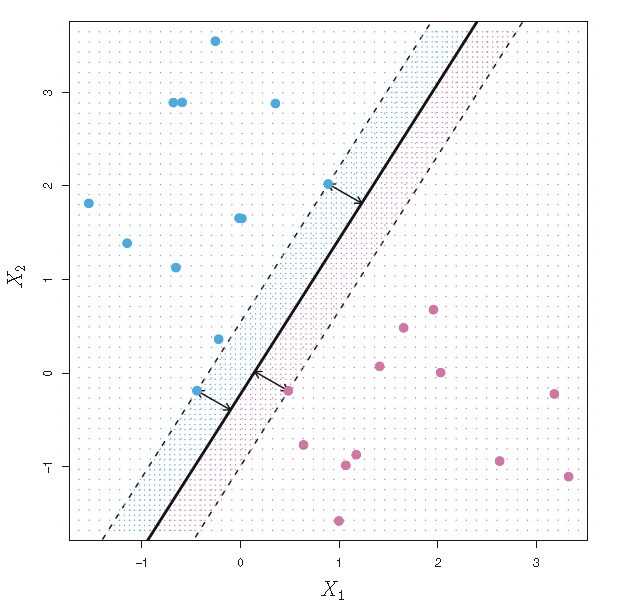
\includegraphics[width=0.3\textwidth]{svm.png}
    \caption{Exemplo de vetores de suporte de 2 dimensões.}
    \label{fig:svm_1}
\end{figure}

\end{frame}

\begin{frame}{CNN}
    Uma rede convolucional é um perceptron multicamada projetado especificamente para reconhecer formas bidimensionais com um alto grau de invariância à tradução, dimensionamento e distorção.

    \begin{figure}[h]
    \centering
    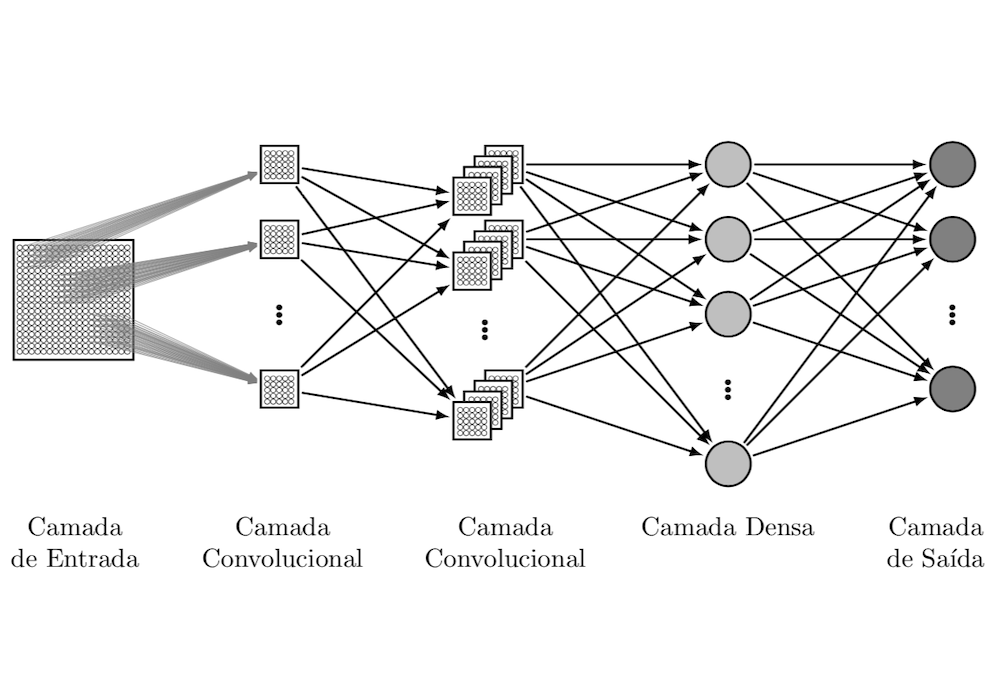
\includegraphics[width=0.5\textwidth]{cnn.png}
    \label{fig:cnn}
    \end{figure}
    
    \begin{itemize}
        \item Mapeamento de características
        \item Retropropagação
        \item Função de hipótese, ativação e otimização
    \end{itemize}
    
\end{frame}

\begin{frame}{EDeN}
    \textit{Explicit Decomposition with Neighborhoods} (EDeN) é um kernel decomposicional de grafos baseado no \textit{Neighborhood Subgraph Pairwise Distance Kernel} (NSPDK) que produz um subgrafo da estrutura secundária de ncRNAs e produz um conjunto explícito de \textit{features} usado para algoritmos de aprendizagem de máquina supervisionados, não-supervisionados ou híbridos de maneira escalável.

    \begin{figure}[h]
    \centering
    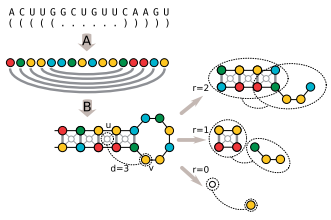
\includegraphics[width=0.4\textwidth]{eden_graph.png}
    \label{fig:eden}
    \caption{Codificação da estrutura secundária de RNA em subgrafos; HEYNE et al. (2012)}
    \end{figure}
    
\end{frame}

\section{Revisão de Literatura}

\begin{frame}{Revisão de literatura}
A construção do estado de conhecimento teve como princípio a análise sistemática de
dissertações, teses, trabalhos científicos e artigos produzidos em um lapso temporal de 6 anos.

\end{frame}
\begin{frame}{Questões de pesquisa}
    \begin{itemize}
   \item QP$_{1}$ Quais os métodos de extração de características em sequências de RNAs?
  \item QP$_{2}$ Quais os modelos matemáticos utilizados na extração?
  \item QP$_{3}$ Quais os grupos de ncRNAs a serem trabalhados e os modelos de aprendizado de máquina aplicados na classificação de snoRNAs?
\end{itemize}
\end{frame}
\begin{frame}{Estratégia de busca}

Para cada base de dados escolhida foram realizadas buscas avançadas em suas ferramentas
de pesquisa com um intervalo de tempo de 6 anos, contemplando como palavras-chaves de pesquisa: \textit{ncRNAs}, \textit{machine learning}, \textit{feature extraction}, \textit{sequence features}, \textit{mathematical approach} às quais resultaram em um conjunto de 292 literaturas.

\end{frame}

\begin{frame}{Critério de Inclusão}
    Para responder as QPs definimos Critérios de Inclusão (CIs) e Critérios de Exclusão (CEs) que irão filtrar os resultados das pesquisas. Os CIs estão listados a seguir.

    \begin{itemize}
  \item CI$_{1}$ Produções científicas que usam os \ac{ncRNAs} como objeto de pesquisa para a extração de características;
  \item CI$_{2}$ Estudos primários que aplicam modelos preditivos supervisionados ou não supervisionados sendo biológico, híbrido ou matemático para classificação de \ac{ncRNAs};
  \item CI$_{3}$ Estudos que classificam as classes e grupos de ncRNAs aplicando o modelo matemático de extração de características;
    \end{itemize}
\end{frame}

\begin{frame}{Critério de Exclusão}
\begin{itemize}
    \item CE$_{1}$ Estudos que não estejam escritos em português ou inglês;
    \item CE$_{2}$ Estudos que a versão completa não é disponível gratuitamente;
    \item CE$_{3}$ Estudos "duplicados", que foram obtidos através da busca em mais de uma base, nestes casos apenas o primeiro será considerado.
    \item CE$_{4}$ Produções científicas que não classificam o grupo de \ac{ncRNAs};
    \item CE$_{5}$ Estudos descritivos de funcionalidades que não discorre sobre a metodologia de \ac{ml} empregue;
\end{itemize}
\end{frame}

\begin{frame}{}
    \begin{table}[h!]
  \begin{center}
    \caption{Resultado das buscas nos bancos de dados}
    \label{tab:table2}
    \begin{tabular}{p{3cm} p{5cm} p{2cm}} % <-- Alignments: 1st column left, 2nd middle and 3rd right, with vertical lines in between
      \hline \\
      \textbf{Base de dados} & \textbf{Palavras-chaves} & \textbf{Produções científicas} \\
      \hline \\
      \textbf{PubMed Central} & \textit{Machine learning, sequence features, ncRNAs} & 98\\
      \textbf{Repositório UnB} & \textit{Machine learning, ncRNAs} & 5 \\
      \textbf{Oxford Academic} & \textit{Machine learning, ncRNAs, mathematic sequence features} & 153\\
      \textbf{Medline} & \textit{Machine learning, ncRNAs, mathematic sequence} & 34\\
      \textbf{SIABI/IFB} & \textit{Machine learning} & 2\\ 
      \hline \\
      \textbf{Total} & & 292  
    \end{tabular}
  \end{center}
\end{table}
\end{frame}

\begin{frame}{Artigo base da tese}
    \begin{itemize}
       \item   \textbf{Bonídia et al. (2021)}  propõe um modelo preditivo matemático para identificação de classes de ncRNAs. Este trabalho foi dividido em três estudos de caso: (I) Avaliação das abordagens matemáticas com os problemas mais frequentes da classe de ncRNAs, por exemplo, \textit{lncRNA versus mRNA}; (II) Teste de generalização em diferentes classificadores de ncRNAs; (III) Análise de persistência em cenários com dados desbalanceados. As técnicas de \ac{ml} aplicadas consistem na transformação discreta de Fourier, mapeamento numérico (representação de Voss, de Real, de z-curve, de EIIP e de números complexos), entropia de Shannon e Tsallis e o uso de redes complexas. 
   \end{itemize}
\end{frame}
\section{Metodologia}

\begin{frame}{Metodologia}
\begin{figure}[h]
\centering
  \caption[Fluxograma de atividades] { Passos da Metodologia}
  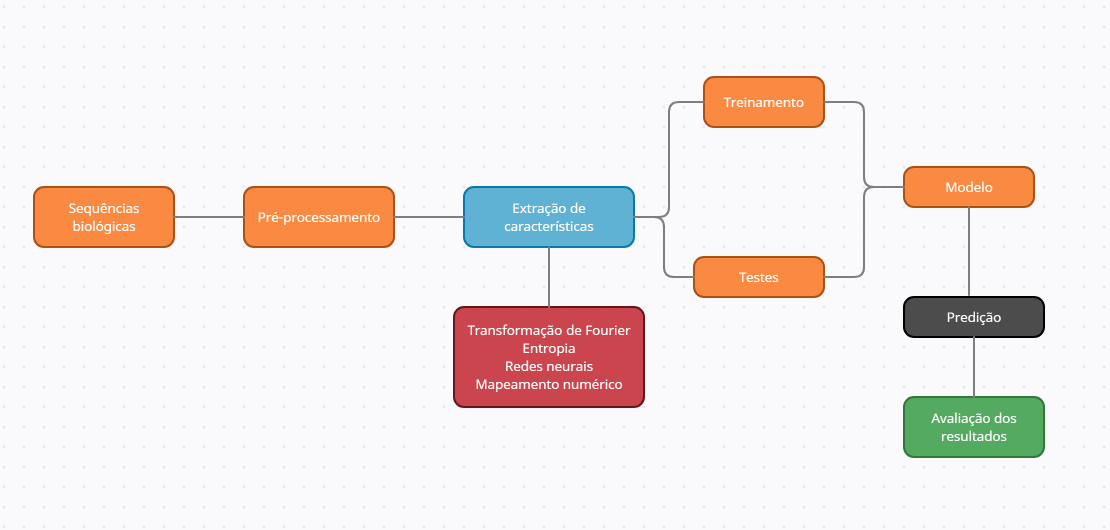
\includegraphics[width=\columnwidth]{fluxograma.png}
  
  \label{fig:research-methodology-thesis}
\end{figure}
\end{frame}

\section{Cronograma}

\begin{frame}{Cronograma}
   \begin{figure}[h]
    \centering
    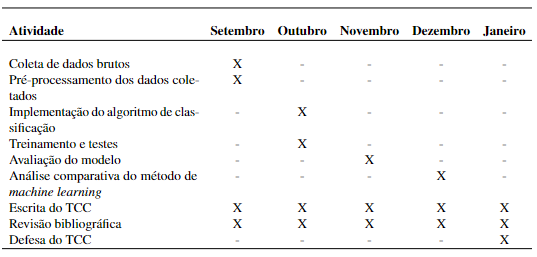
\includegraphics[width=.7\textwidth]{cronograma.png}
    \caption{Cronograma para a relização do TCC.}
    \end{figure}
\end{frame}

\section{Agradecimentos}

\end{document}
